\documentclass{beamer}
\usetheme{Singapore}
\useoutertheme{infolines}  % Información en el pie de página
\usepackage{graphicx}
\usepackage[spanish]{babel}
\usepackage[utf8]{inputenc}
\usepackage{multirow}

\title{Análisis de biospeckle en arándanos}
\author{Laura Velasquez, Juan Montoya}
\institute{FCEN@UdeA}
\date{\today}

\begin{document}

% Portada
\begin{frame}
    \titlepage
\end{frame}

% Introducción
\begin{frame}{Introducción}
    \begin{itemize}
        \item El biospeckle es un fenómeno óptico que ocurre cuando la luz láser incide sobre superficies biológicas activas, como frutas.
        \item Este proyecto analiza el biospeckle en arándanos para evaluar su calidad, distinguiendo entre arándanos óptimos y no óptimos para el consumo.
    \end{itemize}
\end{frame}


% Fundamentos Teóricos
\begin{frame}{Fundamentos Teóricos}
    \begin{itemize}
        \item El speckle es un patrón de interferencia generado por luz coherente reflejada en superficies rugosas.
        \item En tejidos biológicos, el speckle varía con el tiempo (biospeckle) debido al movimiento de las células.
        \\[0.5cm]
        \begin{figure}
            %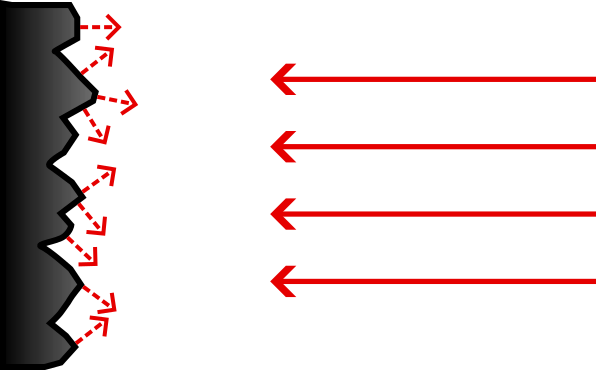
\includegraphics[width=0.35\textwidth]{Superficie.png}
            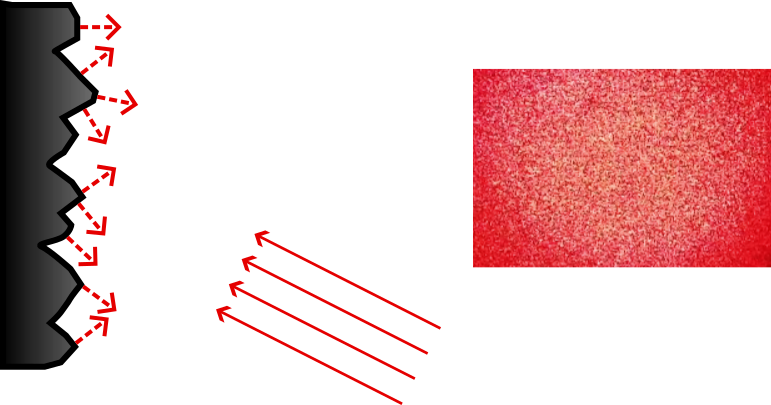
\includegraphics[width=0.65\textwidth]{Observacion.png}
        \end{figure}
    \end{itemize}
\end{frame}

% Montaje Experimental
\begin{frame}{Montaje Experimental}
    \begin{figure}
        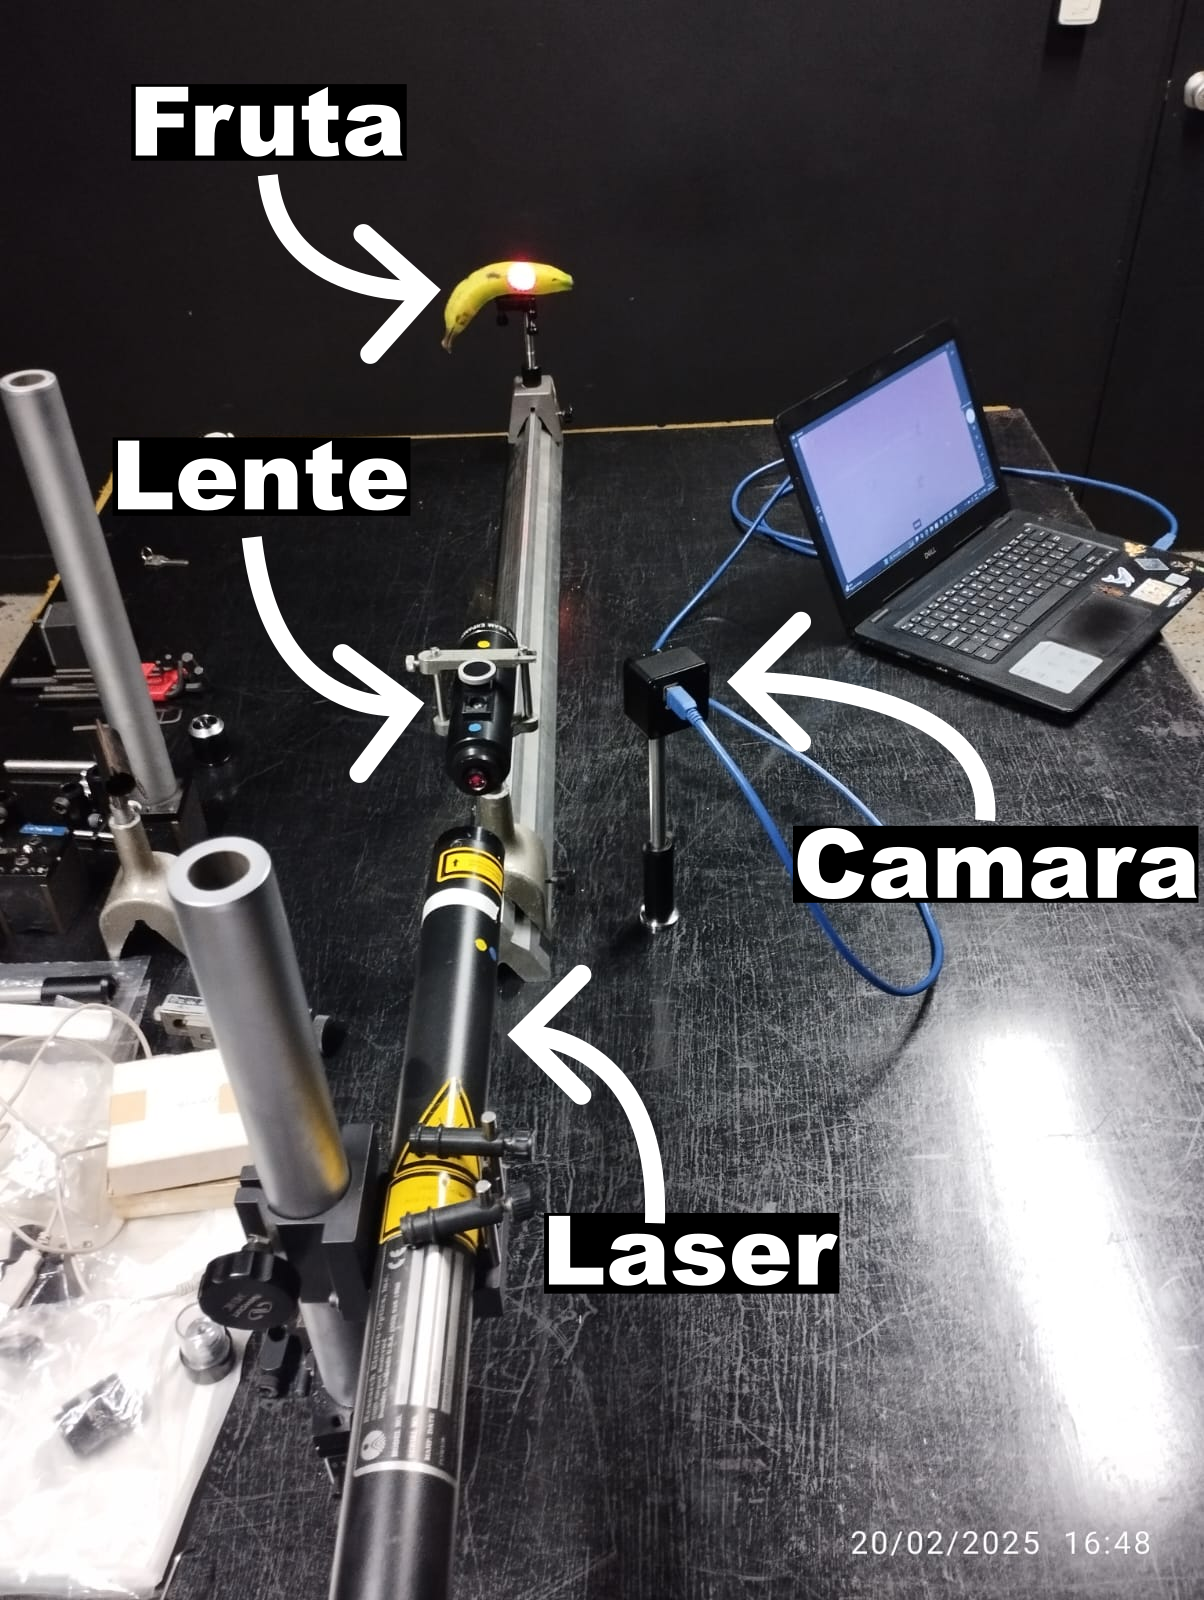
\includegraphics[width=0.4\textwidth]{Bananaforscale.png}
        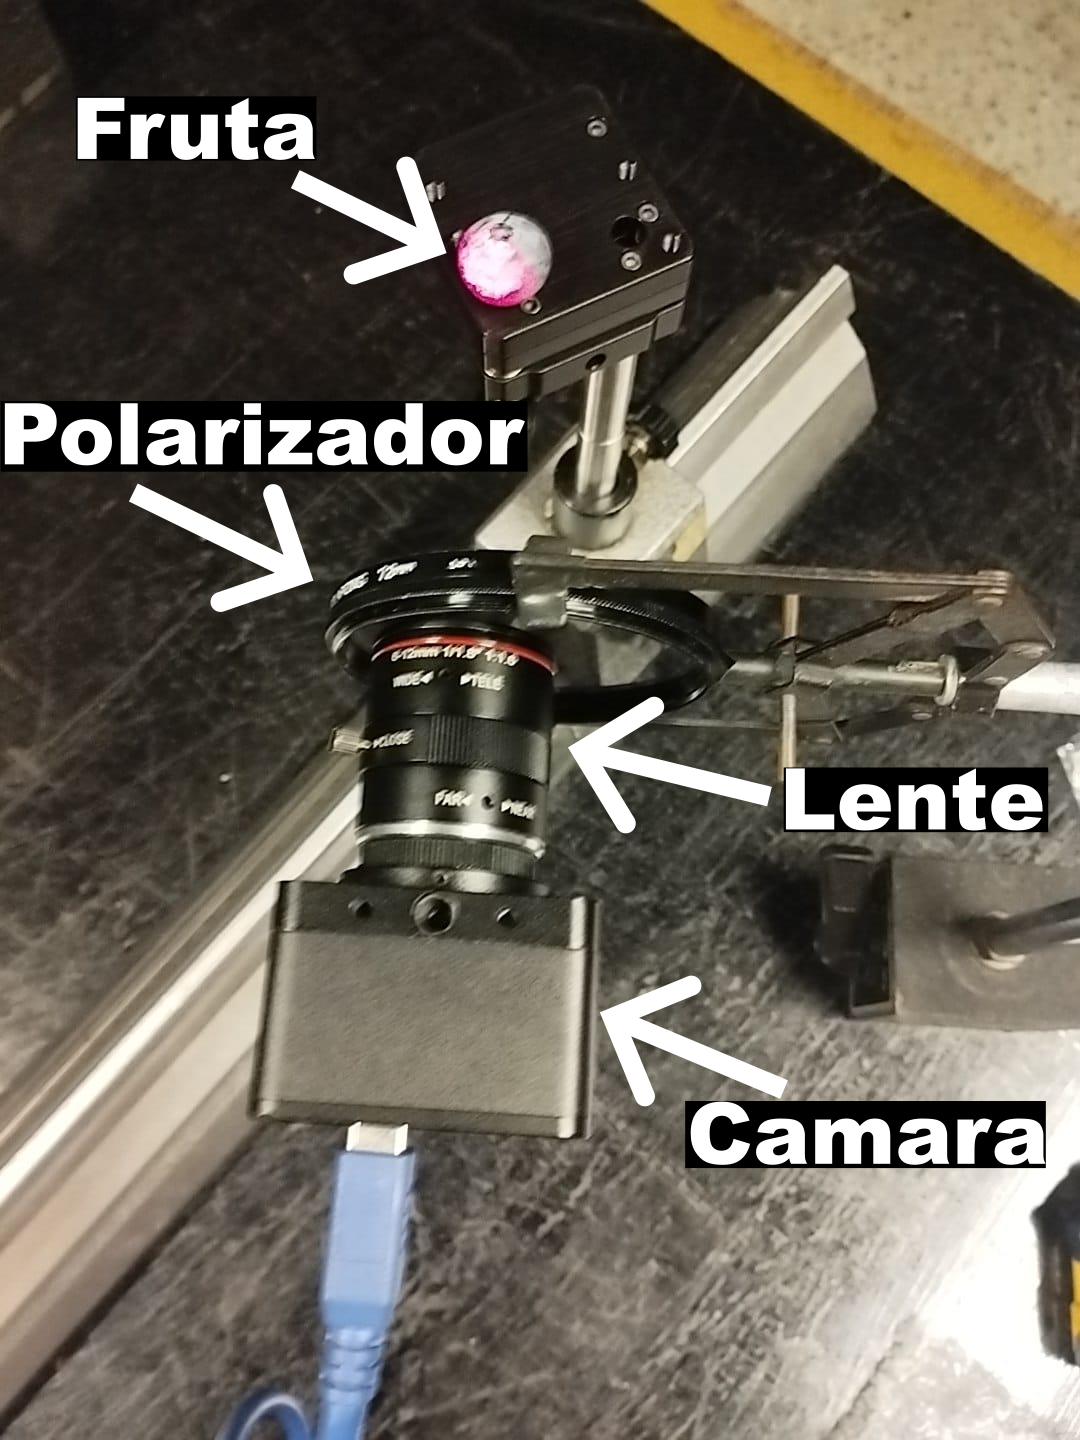
\includegraphics[width=0.4\textwidth]{arandalep.png}
        \caption{Montaje experimental para el análisis de biospeckle en arándanos.}
    \end{figure}
\end{frame}

% Metodología
\begin{frame}{Metodología}
    
    \textbf{Recolección de datos}: Imágenes de biospeckle de 18 arándanos (14 óptimos, 4 no óptimos).
    \begin{figure}
        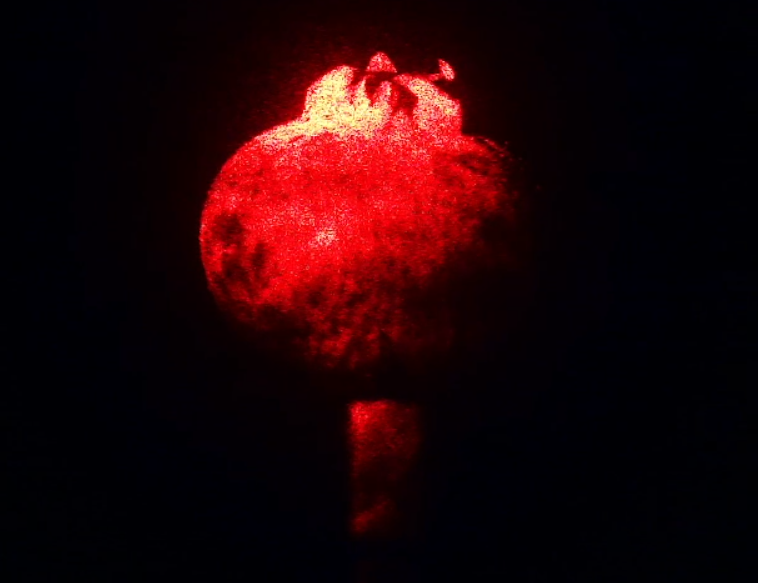
\includegraphics[width=0.4\textwidth]{A5.png}
        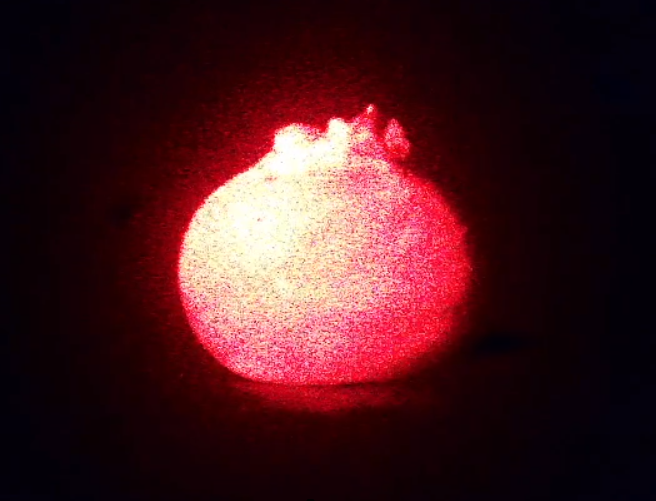
\includegraphics[width=0.4\textwidth]{verde.png}
        \caption{Capturas de pantalla de los videos tomados de los arandanos}
    \end{figure}
\end{frame}

% Metodología
\begin{frame}{Metodología}
    \textbf{Procesamiento}: THSP, matriz de co-ocurrencia y momento de inercia.
    \begin{equation*}
        M_{co} = [N_{i,j}]
    \end{equation*}
    \begin{equation*}
        MI = \sum_{i,j} (i - j)^2 \cdot M_{co}(i,j)
    \end{equation*}
    \begin{equation*}
        DG(x,y) = \sum_{k} \sum_{j} |I_{k}(x,y) - I_{k+l}(x,y)|
    \end{equation*}
\end{frame}

\begin{frame}{Metodología}
    \textbf{Procesamiento}: THSP, matriz de co-ocurrencia y momento de inercia.
    \begin{figure}
        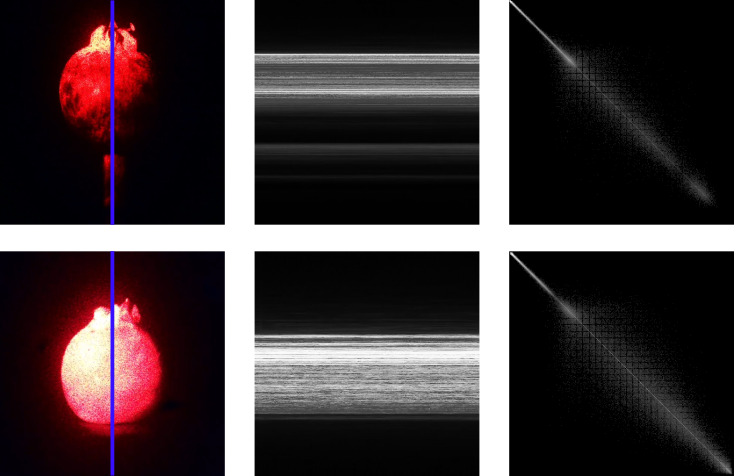
\includegraphics[width=0.8\textwidth]{THSPMCO.png}
    \end{figure}
\end{frame}

% Metodología
\begin{frame}{Metodología}
    \textbf{Procesamiento}: Diferencias generalizadas.
    \begin{figure}
        \includegraphics[width=0.6\textwidth]{Gd.png}
    \end{figure}
\end{frame}

% Metodología
\begin{frame}{Metodología}
    \textbf{Procesamiento}: Cuantificación.
    \begin{figure}
        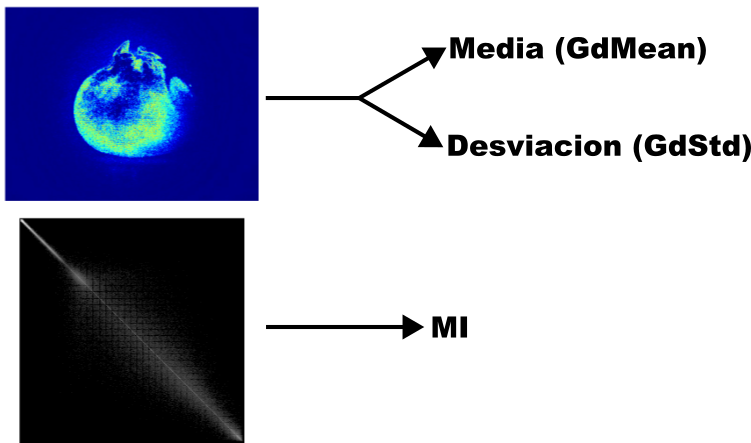
\includegraphics[width=0.6\textwidth]{numeros.png}
    \end{figure}
\end{frame}

% Metodología
\begin{frame}{Metodología}
    \textbf{Análisis estadístico}: 
    \begin{figure}
        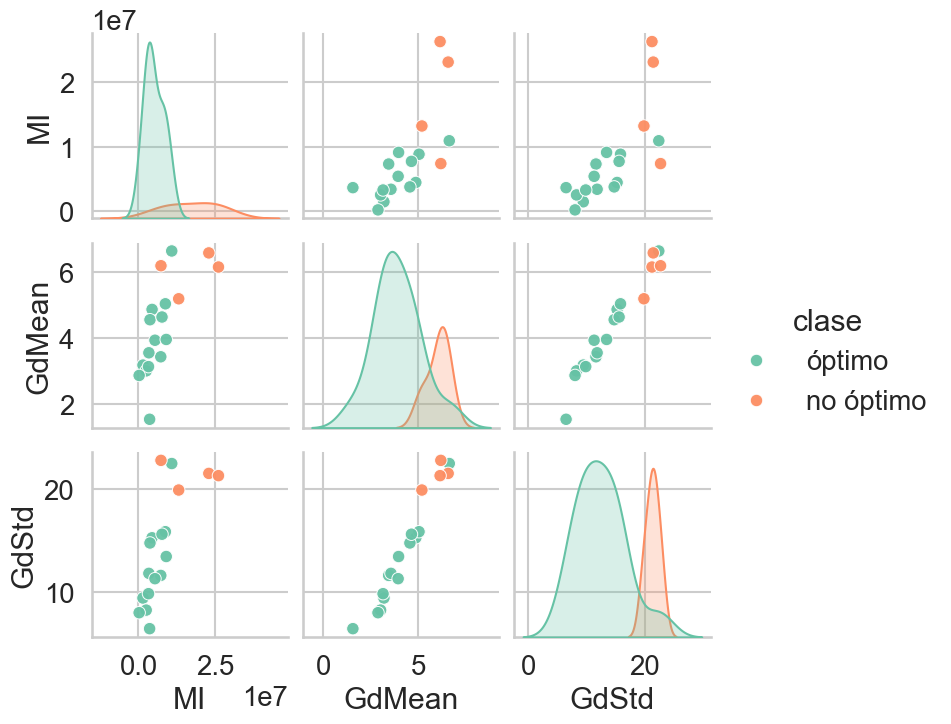
\includegraphics[width=0.7\textwidth]{pairplot.png}
    \end{figure}

\end{frame}

% Resultados
\begin{frame}{Resultados - Análisis Estadístico}
    \begin{table}
        \centering
        \begin{figure}
            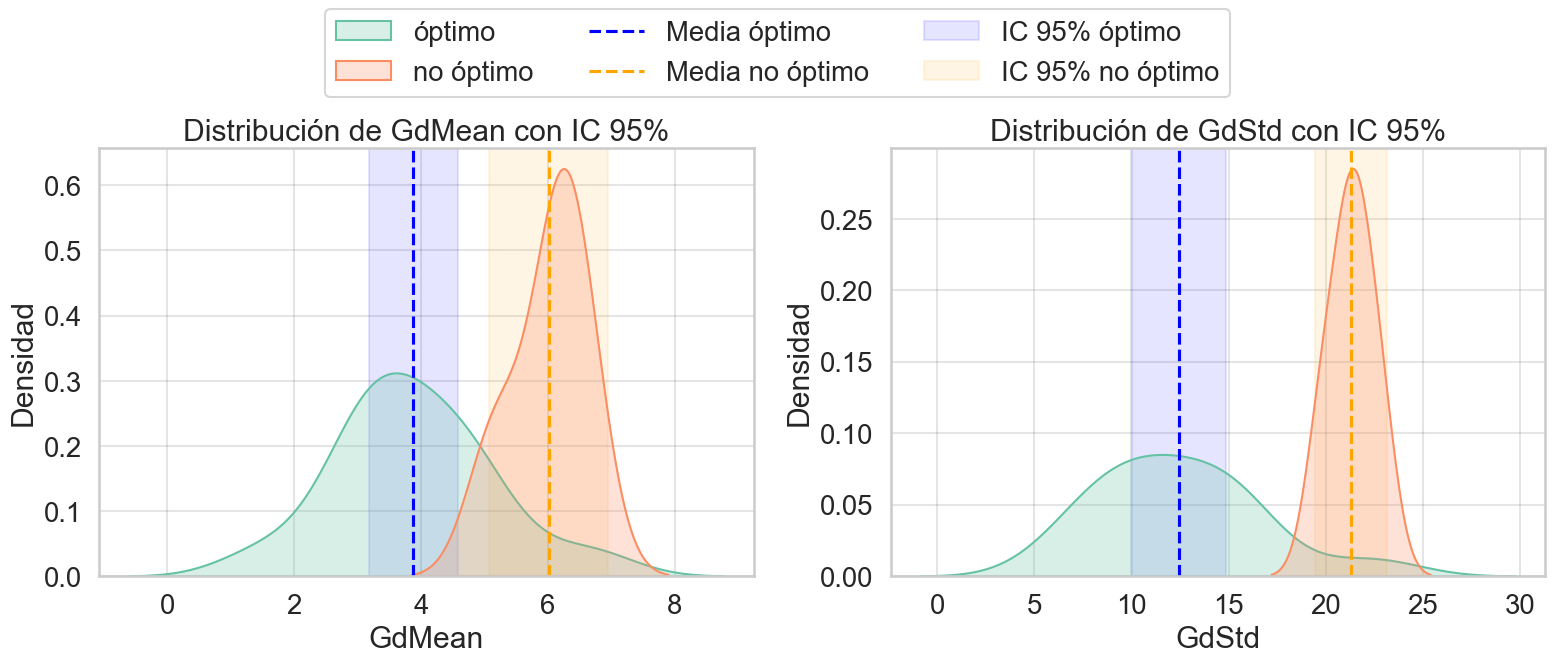
\includegraphics[width=\textwidth]{TGdMeanGdStd.png}
        \end{figure}
        \begin{tabular}{|l|c|c|c|}
            \hline
            \textbf{Variable} & \textbf{p-valor (t-test)} & \textbf{Distinguibles?} & \textbf{IC 95\% óptimo} \\
            \hline
            GdMean & 0.0042 & Sí & [3.2, 4.6] \\
            GdStd & 0.00078 & Sí & [10, 15] \\
            \hline
        \end{tabular}
    \end{table}
\end{frame}

\begin{frame}{Resultados - Análisis Estadístico}
    \begin{table}
        \centering
        \begin{figure}
            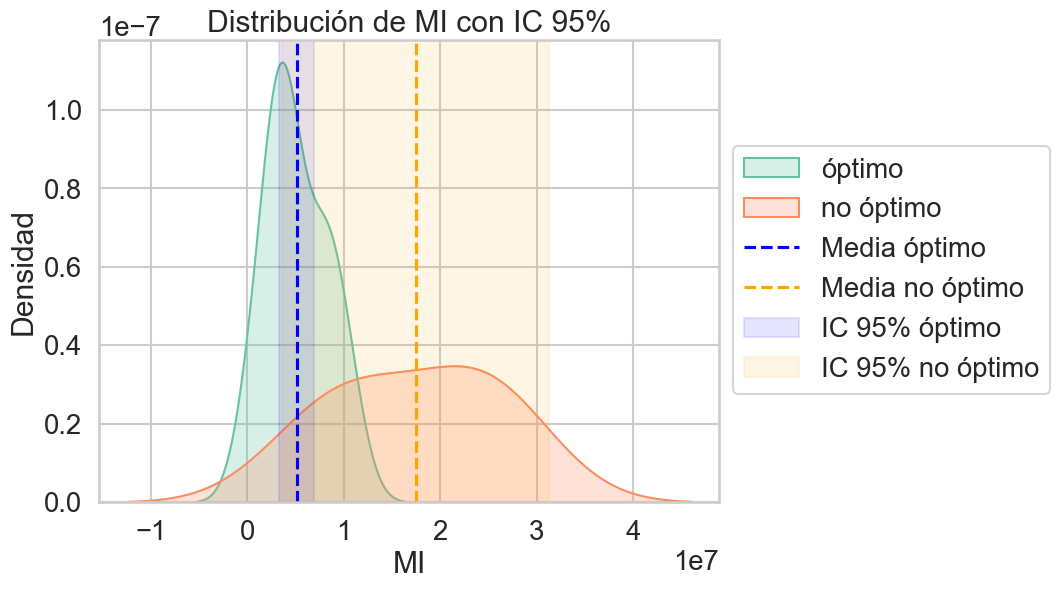
\includegraphics[width=0.85\textwidth]{TMi.png}
        \end{figure}
        \begin{tabular}{|l|c|c|c|}
            \hline
            \textbf{Variable} & \textbf{p-valor (t-test)} & \textbf{Distinguibles?} & \textbf{IC 95\% óptimo} \\
            \hline
            MI & 0.064 & No & [3.3e+06, 7e+06] \\
            \hline
        \end{tabular}
    \end{table}
\end{frame}


\begin{frame}{Resultados - Modelo de Clasificación}
    \begin{itemize}
        \item Modelo de regresión logística con GdMean y GdStd.
        \item \textbf{Precisión}: 89\% (validación cruzada).
        \item \textbf{Matriz de confusión}:
        \begin{figure}
            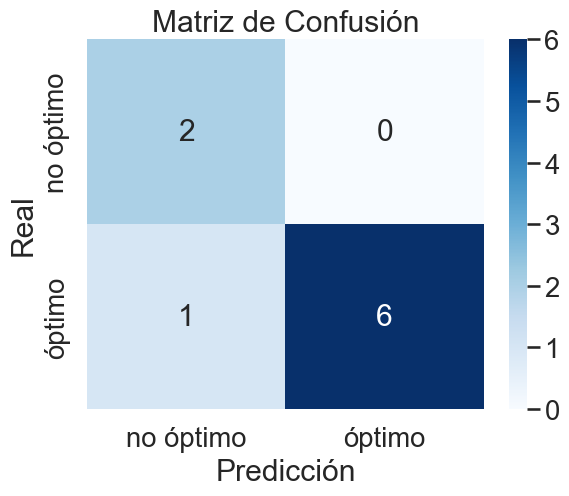
\includegraphics[width=0.45\textwidth]{MConfusion.png}
        \end{figure}
    \end{itemize}
\end{frame}

% Conclusiones
\begin{frame}{Conclusiones}
    \begin{itemize}
        \item El biospeckle es efectivo para evaluar la calidad de arándanos.
        \item GdMean y GdStd son indicadores clave para clasificar arándanos.
        \item El modelo de regresión logística logra un 89\% de precisión.
        \item Para mejorar: Ampliar la muestra para robustecer los resultados.
    \end{itemize}
\end{frame}

% Agradecimientos
\begin{frame}
    \centering
    \Huge{\textbf{Gracias por su atención}}
\end{frame}

\begin{frame}
    \begin{figure}
        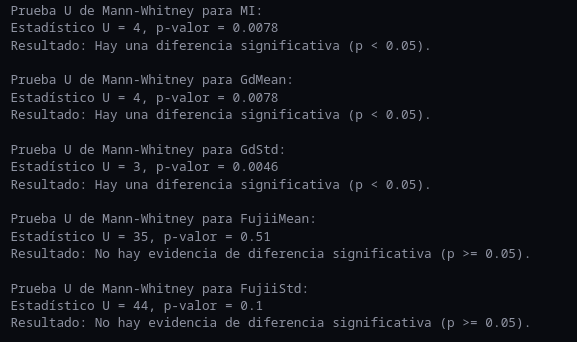
\includegraphics[width =1\textwidth]{whitney.png}
    \end{figure}
\end{frame}

\begin{frame}
    \begin{figure}
        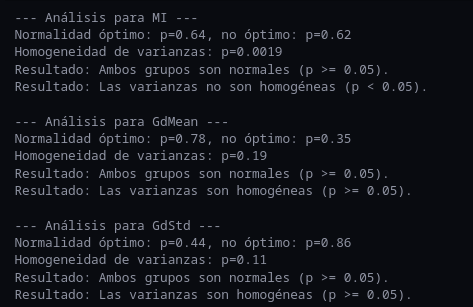
\includegraphics[width=\textwidth]{shapiro.levene.png}
    \end{figure}
\end{frame}

\begin{frame}
    \begin{figure}
        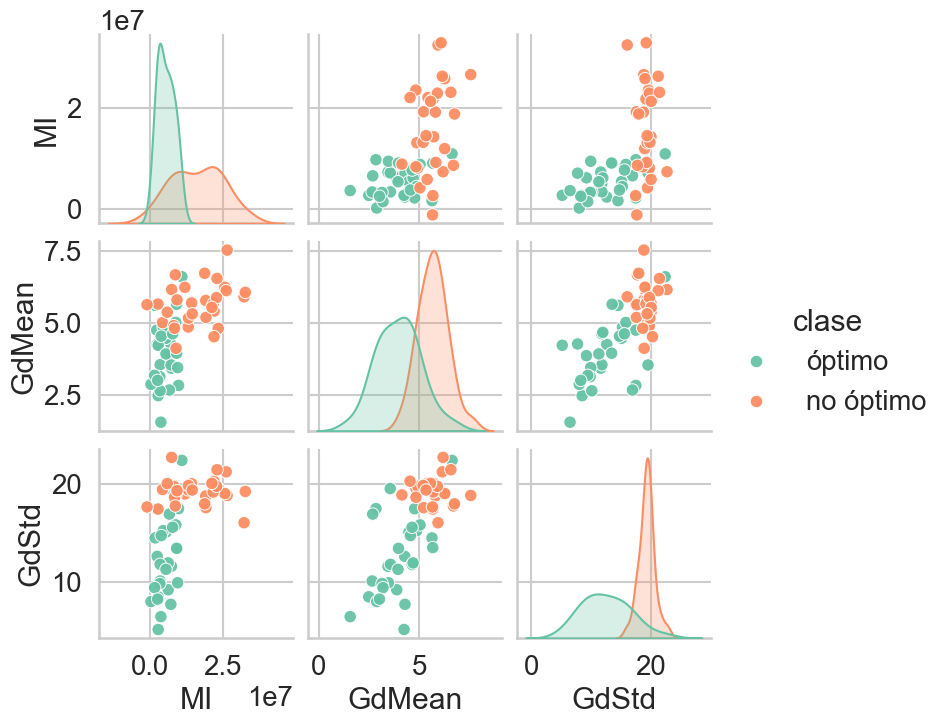
\includegraphics[width=0.9\textwidth]{mcevents.png}
    \end{figure}
\end{frame}

\begin{frame}
    \begin{figure}
        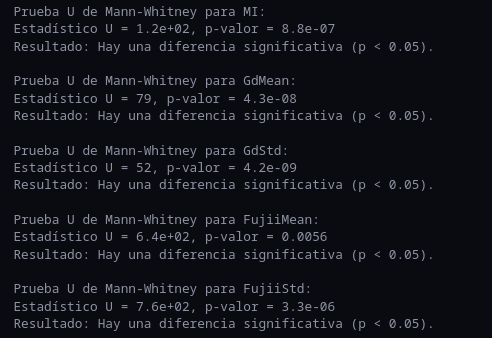
\includegraphics[width=\textwidth]{mcwhitney.png}
    \end{figure}
\end{frame}

\begin{frame}{Mi con monte carlo}
    \begin{table}
        \centering
        \begin{figure}
            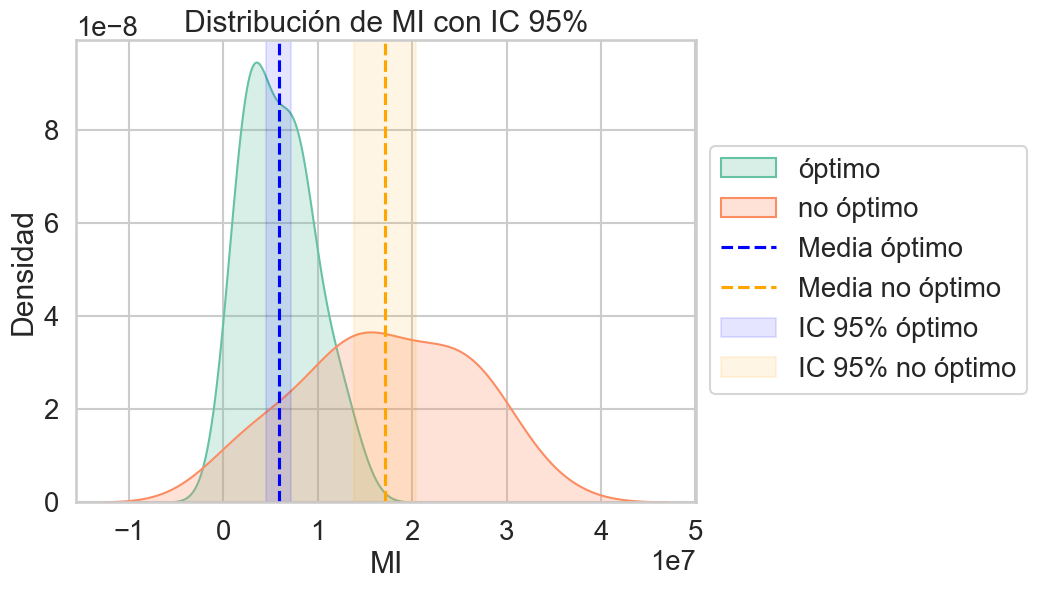
\includegraphics[width=0.85\textwidth]{McMi.png}
        \end{figure}
        \begin{tabular}{|l|c|c|c|}
            \hline
            \textbf{Variable} & \textbf{p-valor (t-test)} & \textbf{Distinguibles?} & \textbf{IC 95\% óptimo} \\
            \hline
            MI & 1.4e-07 & Si & [4.5e+06, 7.2e+06] \\
            \hline
        \end{tabular}
    \end{table}
\end{frame}

\end{document}